\documentclass[11pt]{article}
%%%%%%%%%%%%%%%%%%%%%%%%%%%%%%%%%%%%%%%%%%%%%%%%%%%%%%%%%%%%%%%%%%%%%%%%%%%%%%%
\linespread{1}

\usepackage{amssymb}
\usepackage{amsmath}
\usepackage{xtab}
\usepackage{graphicx}
\usepackage{amsthm}
\usepackage{lscape}
\usepackage{enumitem}
\usepackage{setspace}
\usepackage[margin=0.4 in]{geometry}
\usepackage[english]{babel}
\usepackage[autostyle]{csquotes}
\usepackage{attrib}
\usepackage{booktabs}
\usepackage{mathptmx}
\usepackage[11pt]{moresize}

\usepackage{tabularx}
\usepackage{array}
\usepackage{makecell}
\usepackage[para,online,flushleft]{threeparttable}
\usepackage{tikz}
\usepackage{caption}
\usepackage{titlesec}
\usepackage{setspace}
\usepackage{etoolbox}
\usepackage{csquotes}
\usepackage{anyfontsize}
\usepackage{t1enc}
\usepackage{multirow}
\usepackage{caption}
\usepackage{float}
\usepackage{amssymb}
\usepackage{pdfpages}
\usepackage{natbib}
\usepackage{tabularx}
\usepackage{adjustbox}
\usepackage{url}
\usepackage{graphics}
\bibliographystyle{agsm}
\newcommand{\code}{\texttt}

\setcounter{MaxMatrixCols}{10}
%TCIDATA{OutputFilter=Latex.dll}
%TCIDATA{Version=5.50.0.2953}
%TCIDATA{<META NAME="SaveForMode" CONTENT="1">}
%TCIDATA{BibliographyScheme=Manual}
%TCIDATA{LastRevised=Saturday, December 02, 2017 14:08:59}
%TCIDATA{<META NAME="GraphicsSave" CONTENT="32">}

\def\checkmark{\tikz\fill[scale=0.4](0,.35) -- (.25,0) -- (1,.7) -- (.25,.15) -- cycle;}

\newtheorem{theorem}{Theorem}
\newtheorem{acknowledgement}[theorem]{Acknowledgement}
\newtheorem{algorithm}[theorem]{Algorithm}
\newtheorem{axiom}[theorem]{Axiom}
\newtheorem{case}[theorem]{Case}
\newtheorem{claim}[theorem]{Claim}
\newtheorem{conclusion}[theorem]{Conclusion}
\newtheorem{condition}[theorem]{Condition}
\newtheorem{conjecture}[theorem]{Conjecture}
\newtheorem{corollary}[theorem]{Corollary}
\newtheorem{criterion}[theorem]{Criterion}
\newtheorem{definition}[theorem]{Definition}
\newtheorem{example}[theorem]{Example}
\newtheorem{exercise}[theorem]{Exercise}
\newtheorem{lem}{Lemma}
\newtheorem{proposition}{Proposition}
\newtheorem{hyp}{Hypothesis}
\newcommand\T{\rule{0pt}{3ex}}
\newcommand\B{\rule[-1.5ex]{0pt}{0pt}}
\newcommand{\ts}{\textsuperscript}
\titlespacing*{\subsection} {0pt} {0.1\baselineskip} {0.1\baselineskip}
\titlespacing*{\section}    {0pt} {0.1\baselineskip} {0.1\baselineskip}
\setlength{\belowdisplayskip}{0pt} \setlength{\belowdisplayshortskip}{0pt}
\setlength{\abovedisplayskip}{0pt} \setlength{\abovedisplayshortskip}{0pt}
\pagenumbering{gobble}

\usepackage[document]{ragged2e}
\setlength{\RaggedRightParindent}{\parindent}

%%%%%%%%%%%%%%%%%%%%%%%%%%%%%%%%%%%%%%%%%%%%%%%%%%%%%%%%%%%%%%%%%%%%%%%%%%%%%%%

\begin{document}
\begin{center}

\begin{figure}
 \center
  \caption{ROC score distribution for selection model}
  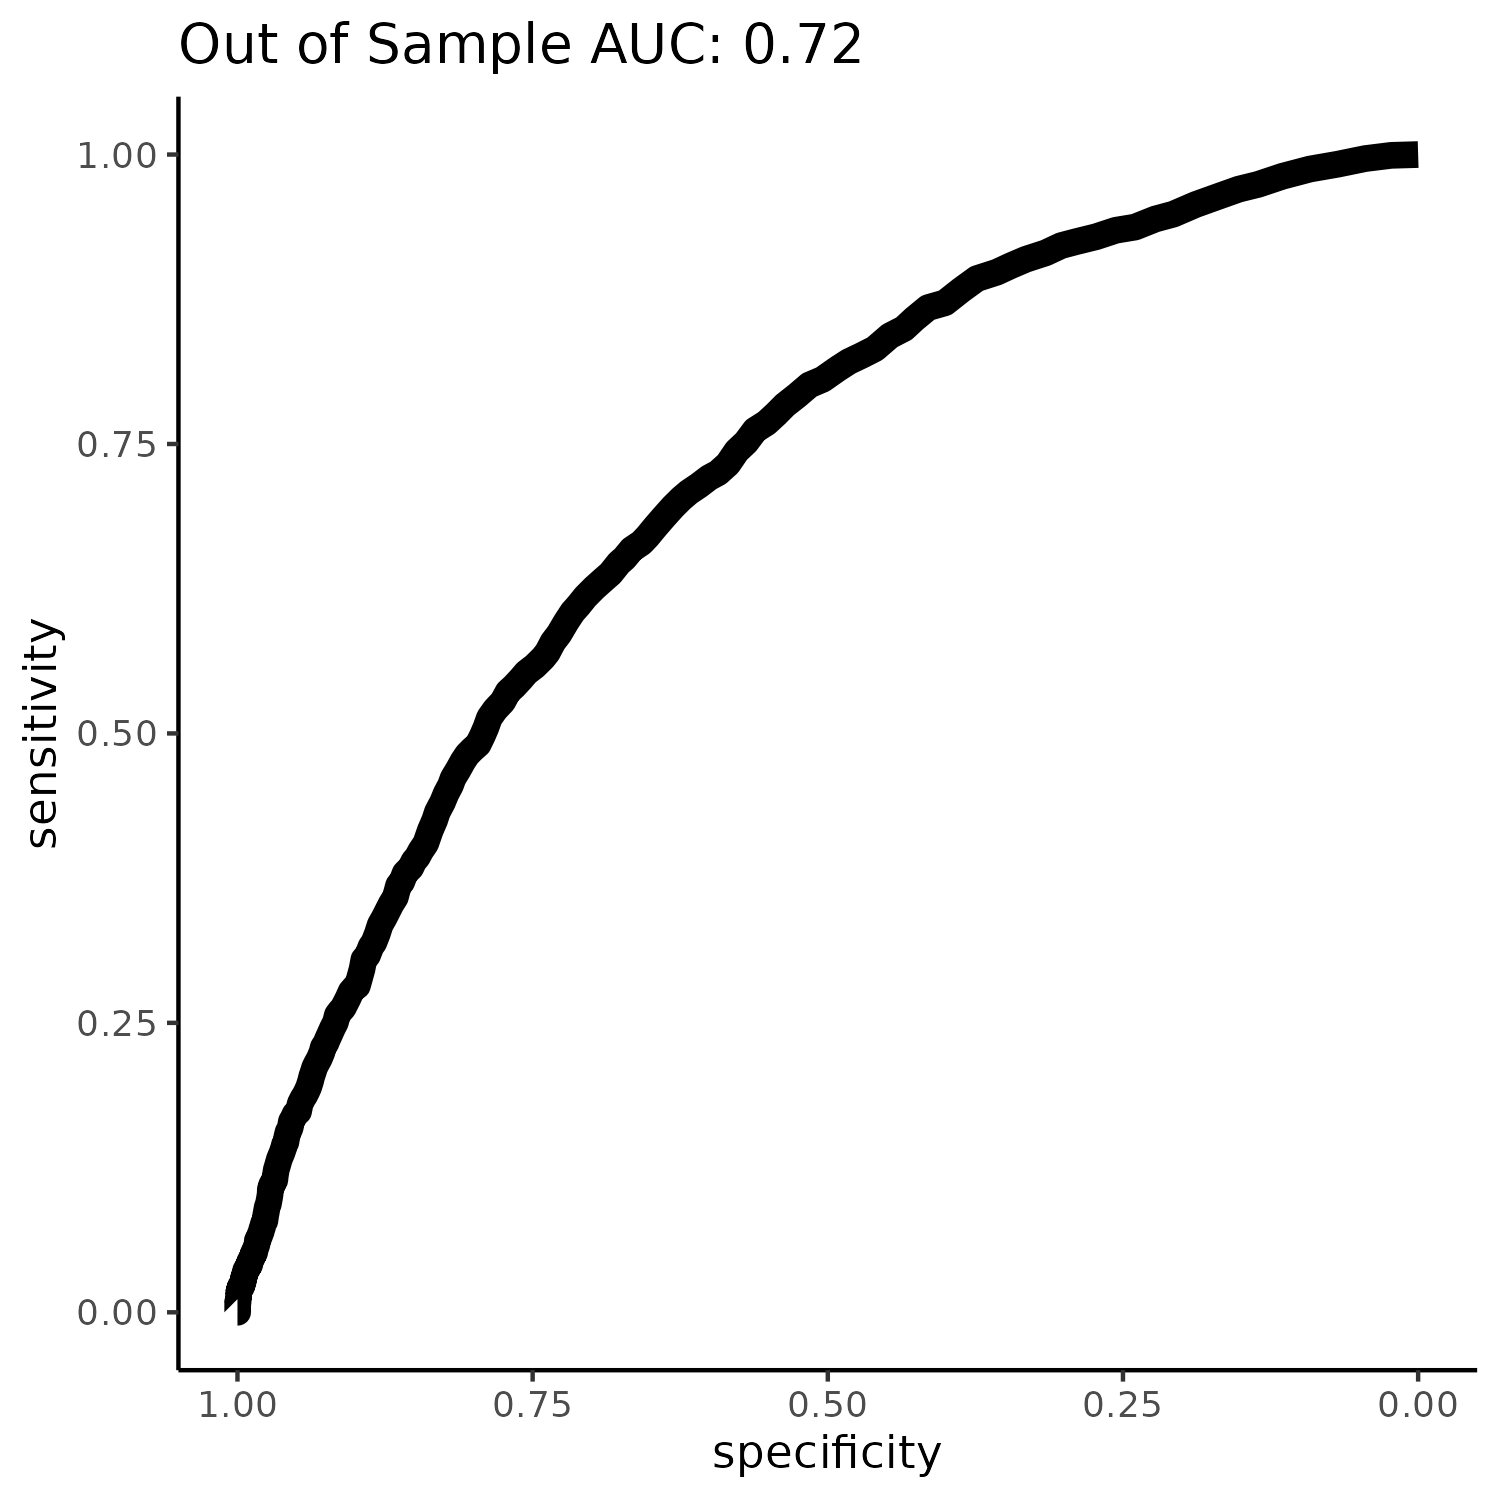
\includegraphics[width=.4\textwidth]{roc_graph.png}
  \caption*{\footnotesize \emph{Notes:} This figure reports the out-of-sample ROC score of a random forest model using a set of high dimensional startup observables to predict the probability that a venture capitalist has funded a startup's early stage round, in a sample of startups that received early stage financing.}
\end{figure}

\begin{figure}
  \center
  \caption{Histogram of Predictions}
  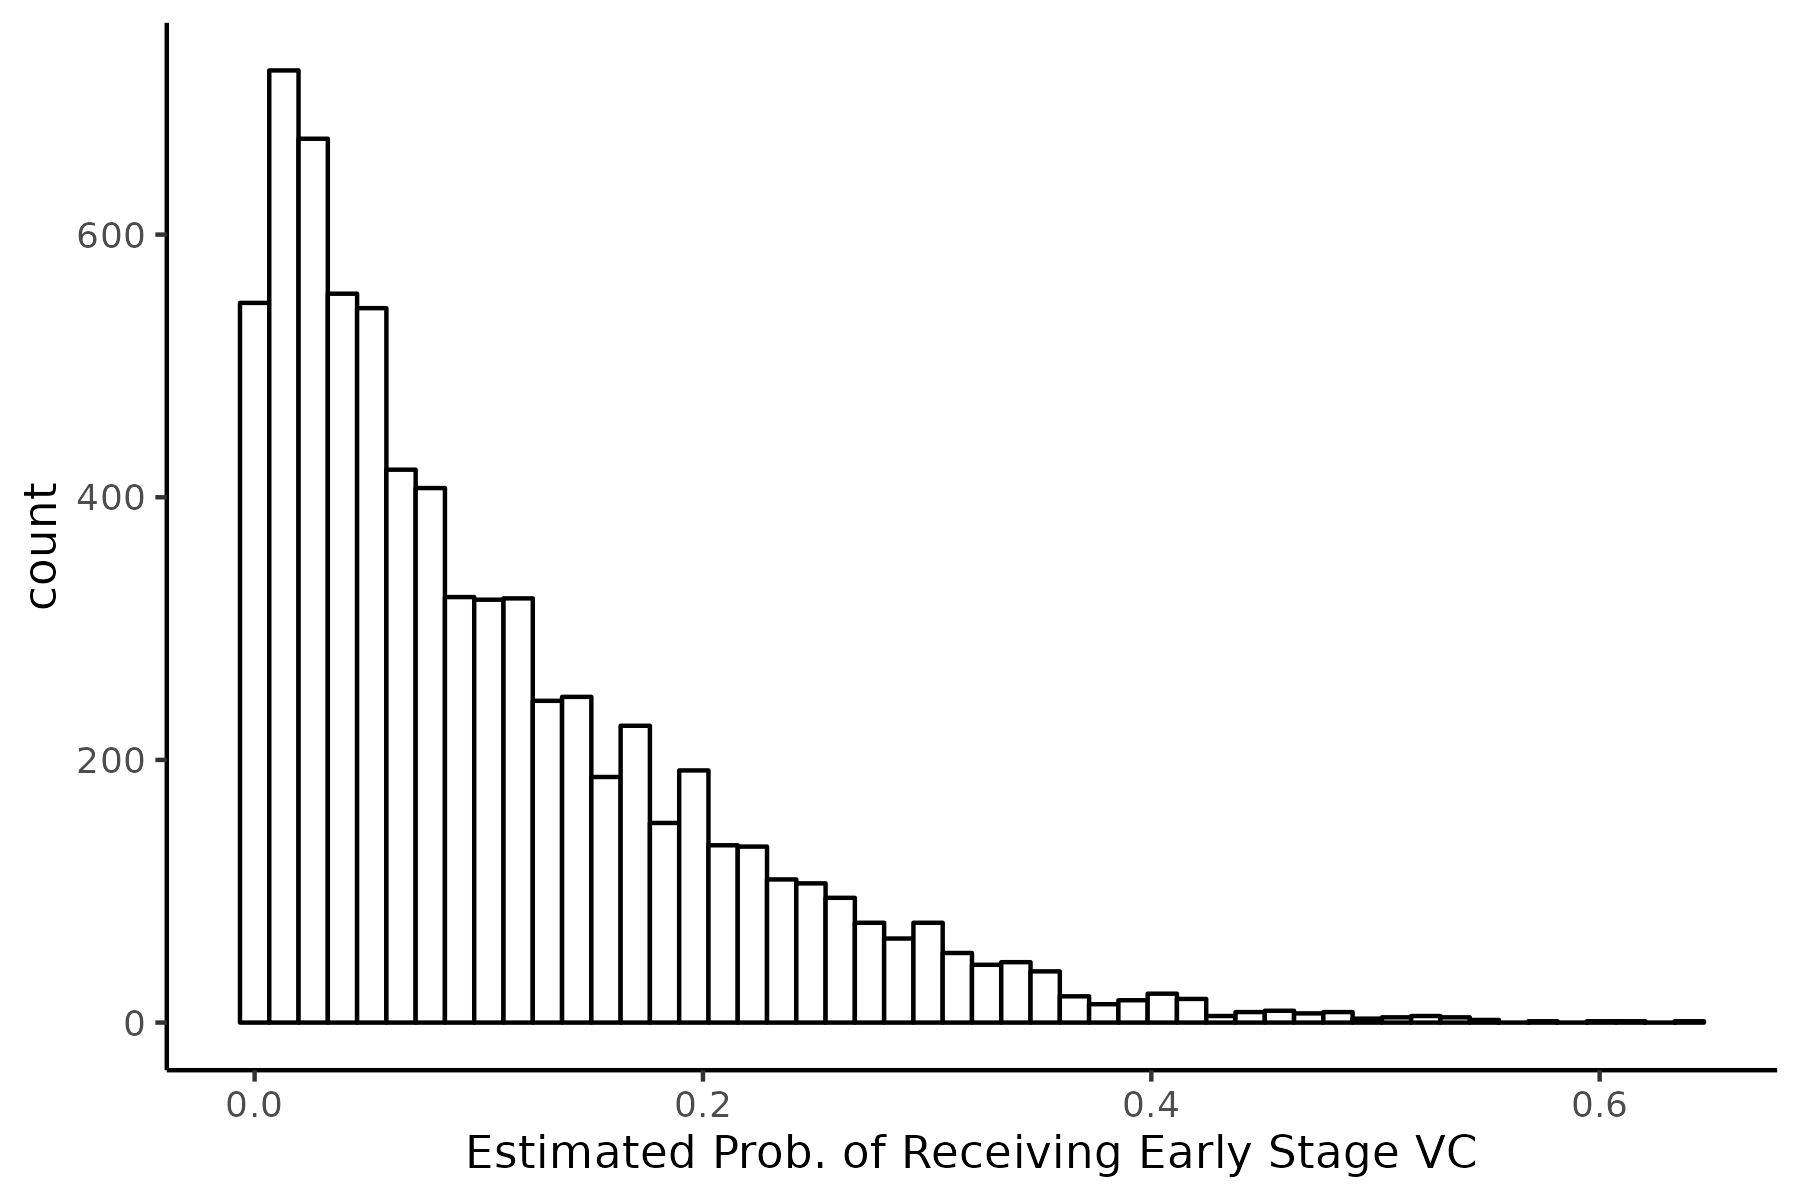
\includegraphics[width=.8\textwidth]{pred_histogram.png}
    \caption*{\footnotesize \emph{Notes:} This figure reports the histogram of out of sample predicted probability of receiving venture capital financing from a random forest model using a set of high dimensional startup observables, in a sample consisting only of startups that received early stage financing.}
\end{figure}

%%%%%%%%%%%%%%%%%%%%%%%%%%%%%%%%%%%%%%%%%%%%%%%%%%%%%%%%%%%%%%%%%%%%%%%%%%%%%%%

\begin{figure}
  \caption{Binned scatterplot for outcomes across the distribution of predicted probability of venture capital}
  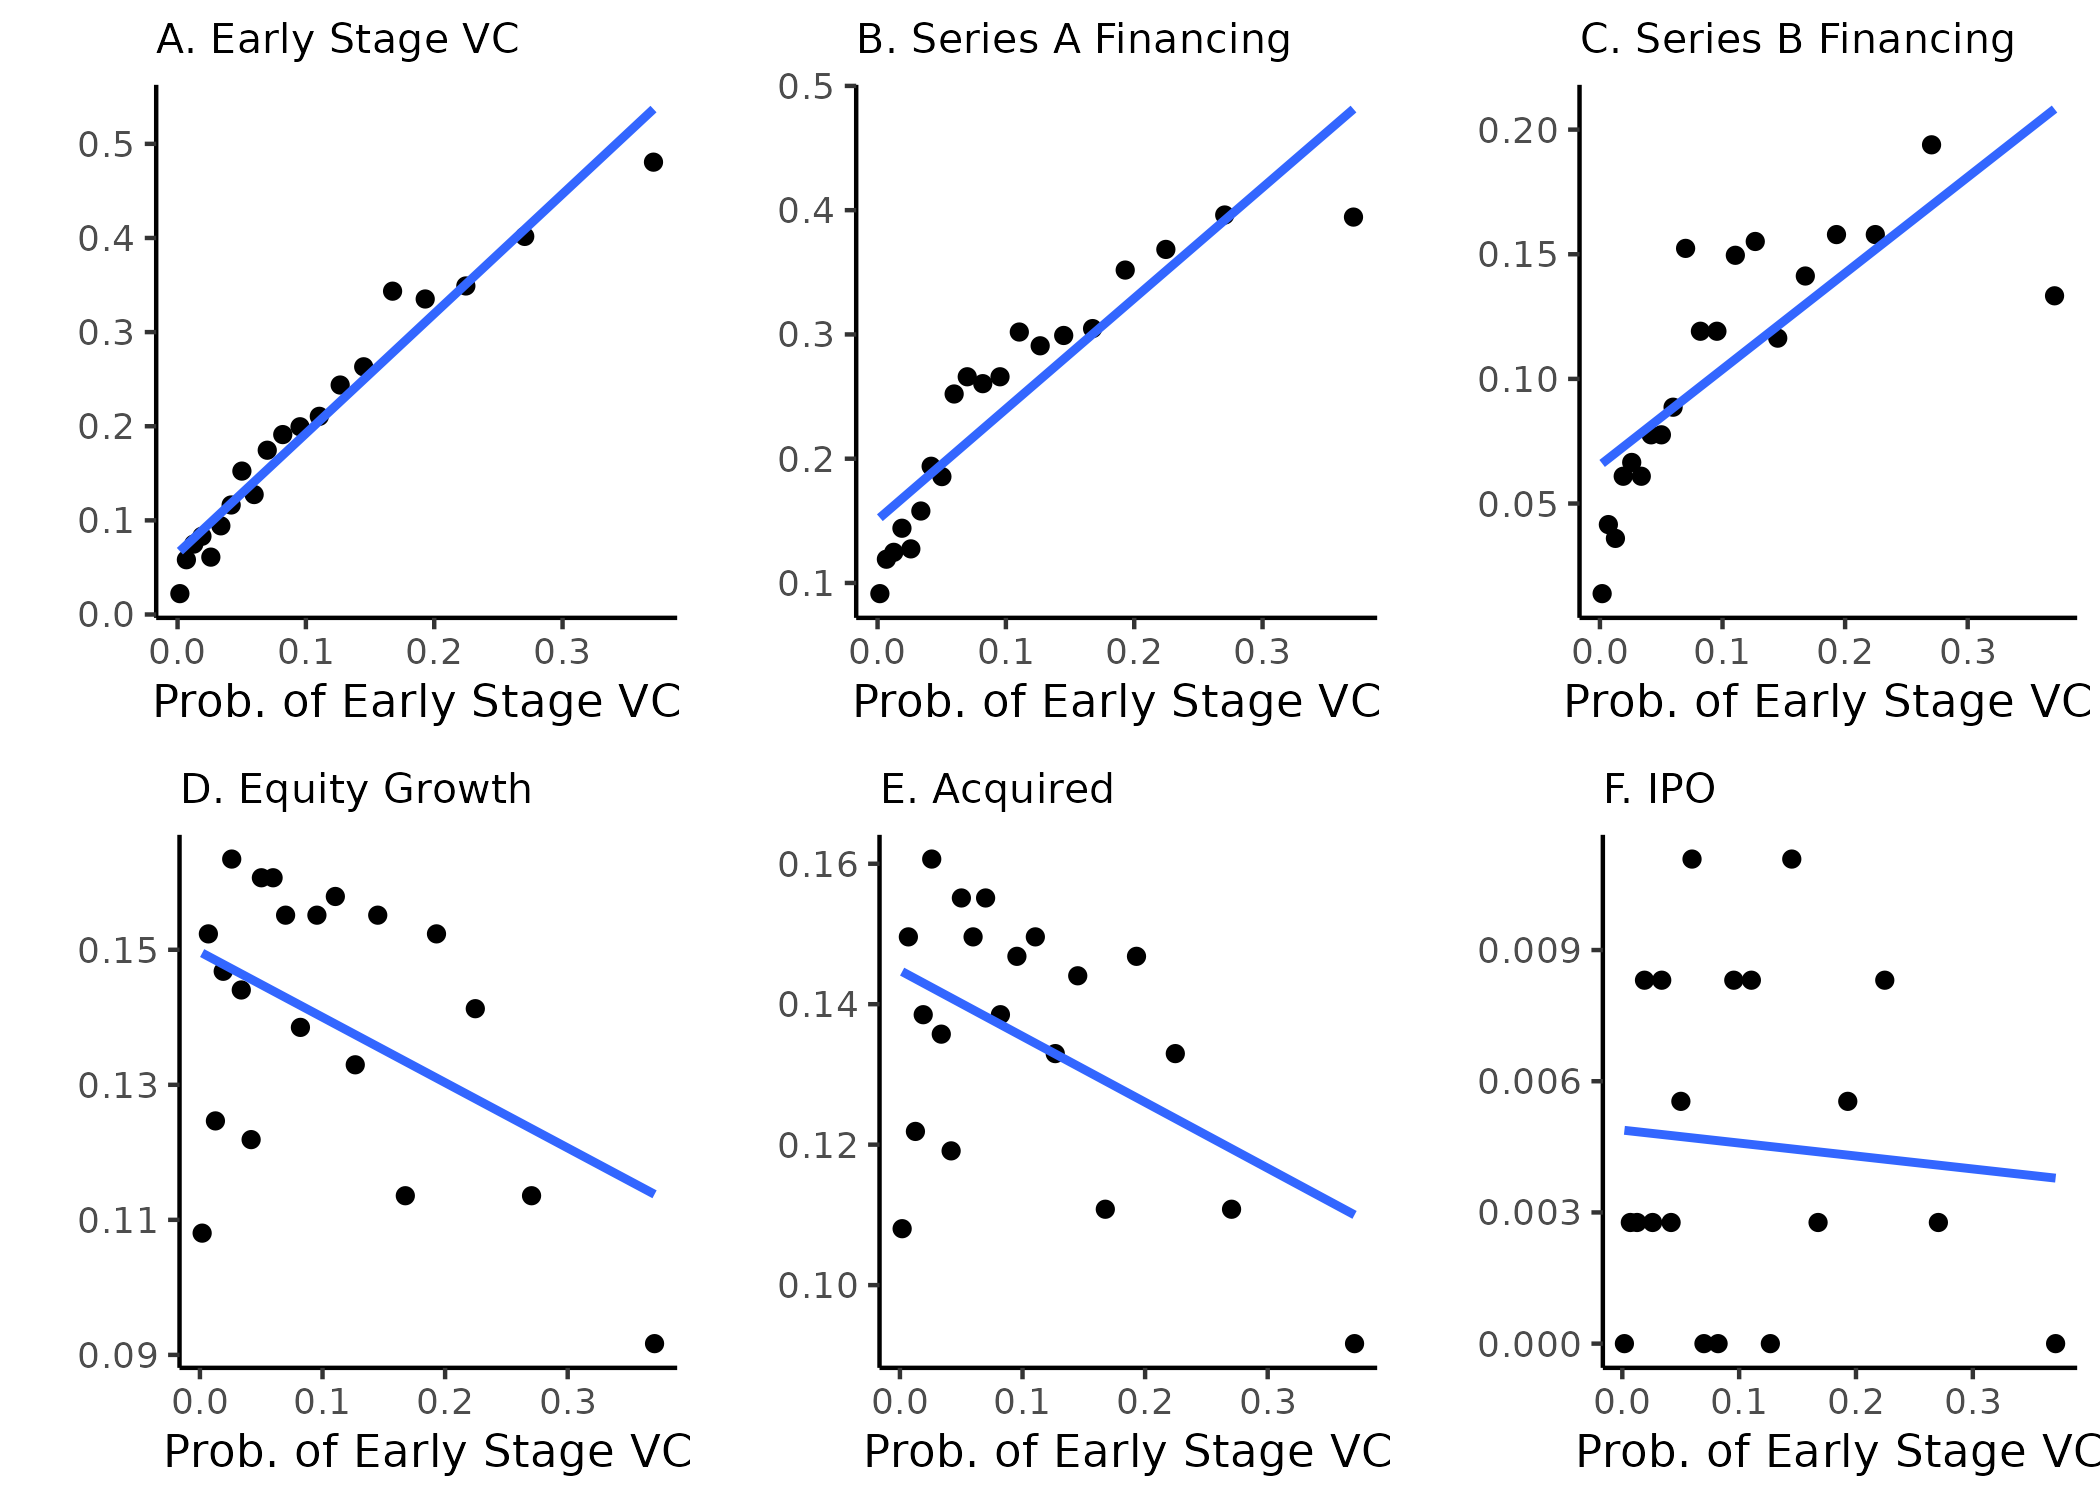
\includegraphics[width=.85\textwidth]{binscatters_p_vc_by_outcome.png}
      \caption*{\footnotesize \emph{Notes:} This figure plots binned scatterplots on the out of sample predicted probability of receiving venture capital from our random forest model. The relationship between this probability and the receipt of VC is positive, but the relationship to other outcomes is more nuanced. }

\end{figure}

\begin{figure}
 \caption{Distribution of treatment effects}
  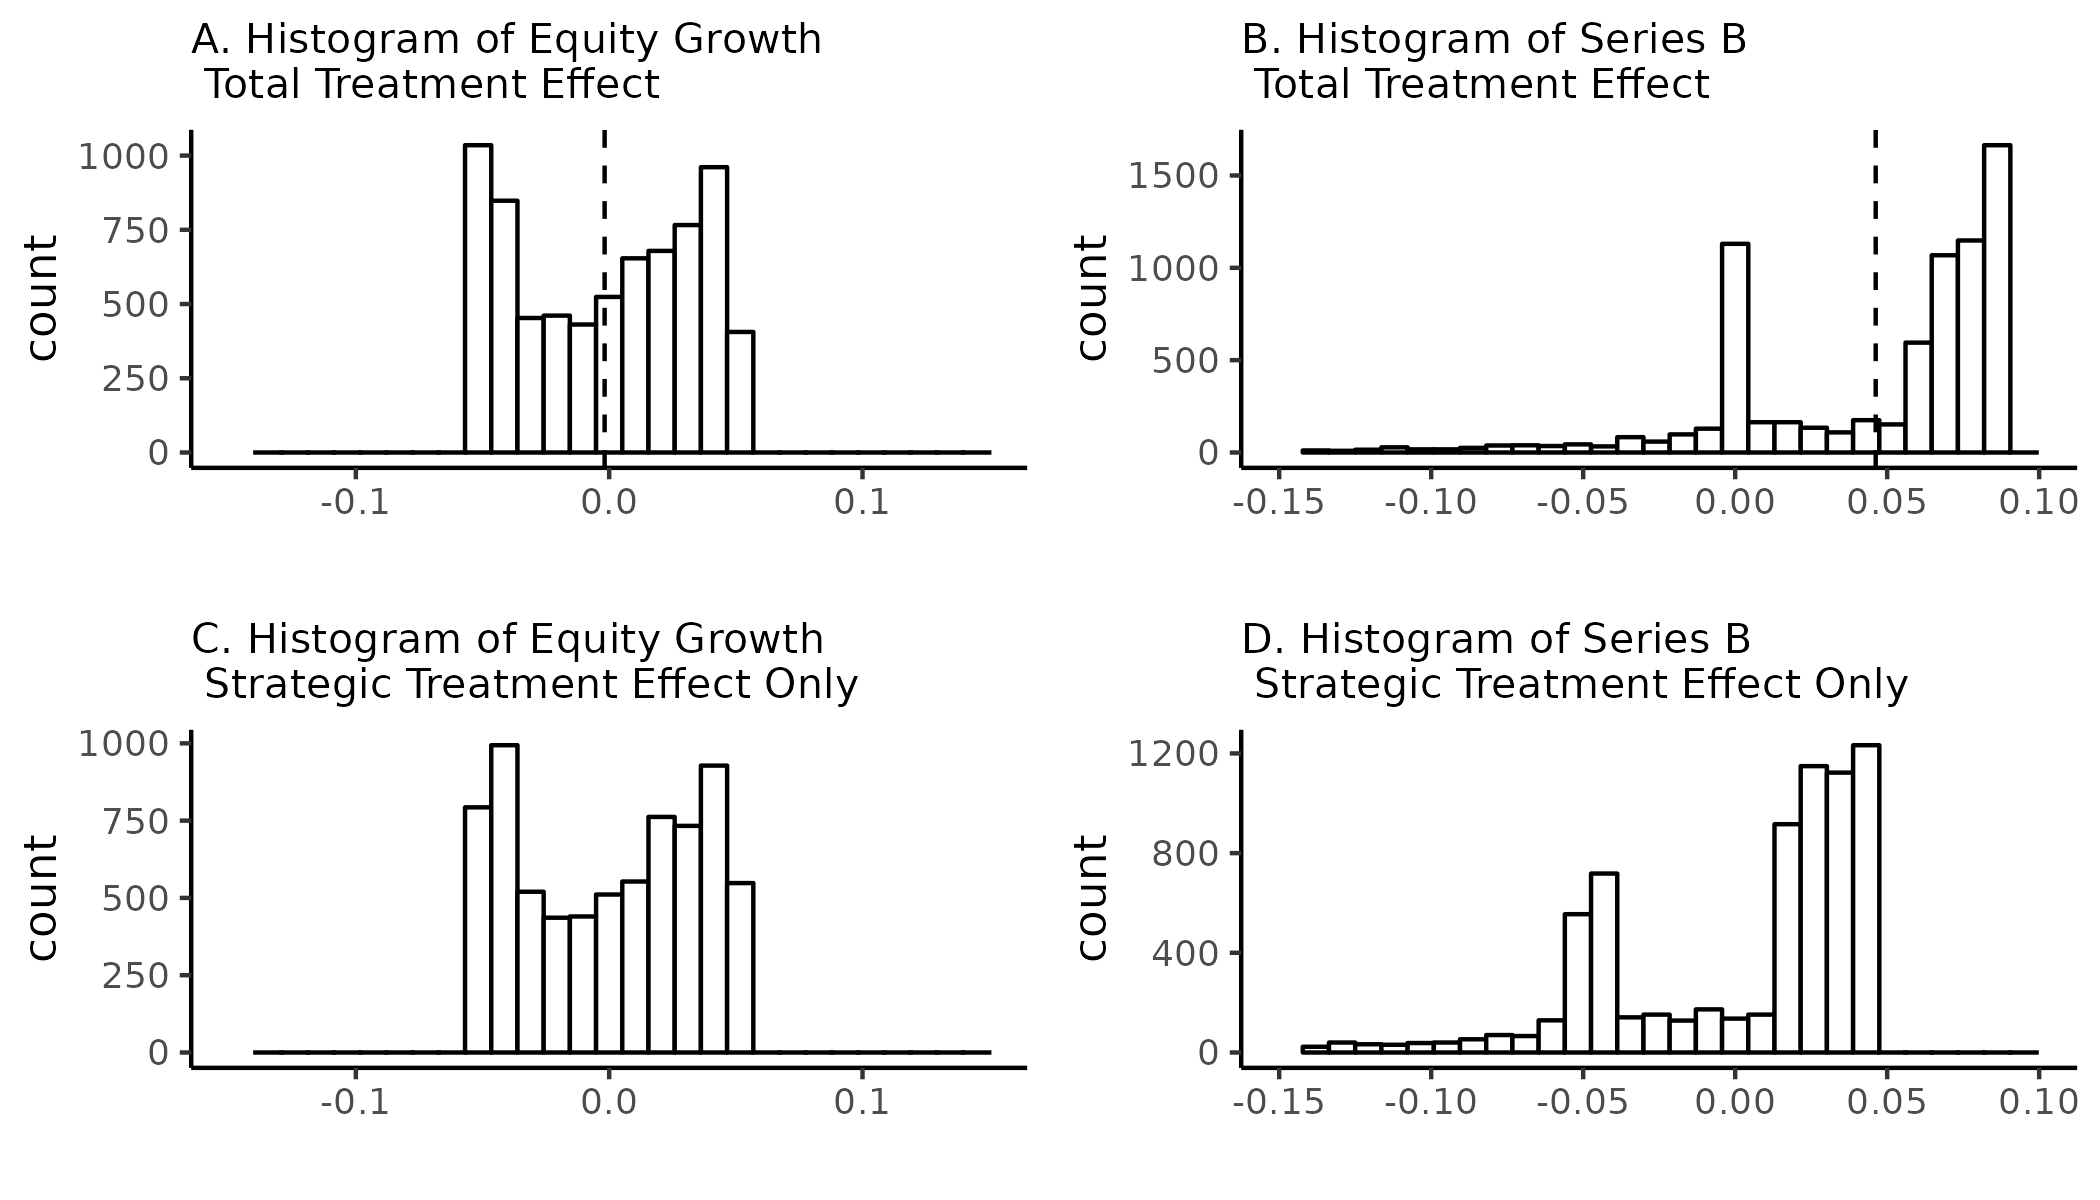
\includegraphics[width=.85\textwidth]{dist_treatment_effect.png}
      \caption*{\footnotesize \emph{Notes:} This figure reports estimated treatment effects ($\hat{\Delta}$) for the firms in our sample. The dashed line in panels A and B represent the mean treatment effect for firms. }

\end{figure}

%%%%%%%%%%%%%%%%%%%%%%%%%%%%%%%%%%%%%%%%%%%%%%%%%%%%%%%%%%%%%%%%%%%%%%%%%%%%%%%

\clearpage
\newpage

\begin{table}[htp]
\begin{center}
\caption{Summary Statistics}


    \begin{threeparttable}


% Table created by stargazer v.5.2.3 by Marek Hlavac, Social Policy Institute. E-mail: marek.hlavac at gmail.com
% Date and time: Wed, Jul 27, 2022 - 11:02:48 AM
\begin{tabular}{@{\extracolsep{5pt}}lccc} 
\\[-1.8ex]\hline 
\hline \\[-1.8ex] 
Statistic & \multicolumn{1}{c}{Mean} & \multicolumn{1}{c}{St. Dev.} & \multicolumn{1}{c}{N} \\ 
\hline \\[-1.8ex] 
Amount Raised Total & 11,592,973.000 & 71,123,260.000 & 7,219 \\ 
Seed Amount Raised & 1,309,721.000 & 1,512,657.000 & 7,219 \\ 
Angel Funding Amount Raised & 114,929.200 & 452,395.500 & 7,219 \\ 
Early Stage Amount Raised & 1,593,344.000 & 1,608,507.000 & 7,219 \\ 
Series A Amount Raised & 1,923,141.000 & 4,852,012.000 & 7,219 \\ 
Series B Amount Raised & 2,150,582.000 & 8,973,669.000 & 7,219 \\ 
Seed VC & 0.187 & 0.390 & 7,219 \\ 
Pre Seed VC & 0.008 & 0.088 & 7,219 \\ 
Early Stage VC & 0.199 & 0.399 & 7,219 \\ 
Equity Growth & 0.139 & 0.346 & 7,219 \\ 
IPO & 0.005 & 0.067 & 7,219 \\ 
Acquisition & 0.135 & 0.342 & 7,219 \\ 
\hline \\[-1.8ex] 
\end{tabular} 

\begin{tablenotes}
\item {\footnotesize
\emph{Notes:} Data represents U.S. based firms in Crunchbase founded between 2005 and 2017 that raised a form of eary stage financing, defined as any of a seed round, a pre-seed round, crowdfunding, angel, or grants. \emph{Seed VC} is an indicator equal to 1 if the startup receives seed financing from a venture capitalist. \emph{Early Stage VC} is an indicator equal to 1 if the startup receives any form of early stage financing from a venture capitalist. \emph{Equity Growth} is an indicator equal to 1 if the startup achieves an equity through either IPO or Acquisition.}
\end{tablenotes}
  \end{threeparttable}

\end{center}
\end{table}



\begin{table}[htp]
\begin{center}
\caption{Strategic Determinant Function: Top Features for Strategic Treatment Effect of VC on Equity Growth}

    \begin{threeparttable}


% Table created by stargazer v.5.2.3 by Marek Hlavac, Social Policy Institute. E-mail: marek.hlavac at gmail.com
% Date and time: Wed, Jul 27, 2022 - 11:02:25 AM
\begin{tabular}{@{\extracolsep{5pt}}lcccccc} 
\\[-1.8ex]\hline 
\hline \\[-1.8ex] 
 & \multicolumn{6}{c}{\textit{Dependent variable:}} \\ 
\cline{2-7} 
\\[-1.8ex] & \multicolumn{4}{c}{Equity Growth} & \multicolumn{2}{c}{Raised Series B} \\ 
 & OLS & Double LASSO & OLS & Double LASSO & OLS & Double LASSO \\ 
\\[-1.8ex] & (1) & (2) & (3) & (4) & (5) & (6)\\ 
\hline \\[-1.8ex] 
 Early Stage VC & 0.025$^{*}$ & $-$0.011 &  &  & 0.091$^{***}$ & 0.046$^{***}$ \\ 
  & (0.014) & (0.015) &  &  & (0.015) & (0.013) \\ 
  & & & & & & \\ 
 Seed VC &  &  & 0.026$^{*}$ & $-$0.010 &  &  \\ 
  &  &  & (0.014) & (0.014) &  &  \\ 
  & & & & & & \\ 
\hline \\[-1.8ex] 
Observations & 7,219 & 7,219 & 7,219 & 7,219 & 7,219 & 7,219 \\ 
R$^{2}$ & 0.095 & 0.147 & 0.095 & 0.150 & 0.053 & 0.106 \\ 
\hline 
\hline \\[-1.8ex] 
\end{tabular} 

  \begin{tablenotes}
      \item {\footnotesize
        \emph{Notes:} Estimates the impact of early stage venture capital on firm
  outcomes. Columns (1), (3), and (5) report naive OLS estimators with no
  controls. Columns (2), (4), and (6) report estimates using the double LASSO
  approach of Belloni et al (2014). Founding year fixed effects are included in all regressions. Standard errors clustered at the state level are reported. $^{*}$p$<$0.1; $^{**}$p$<$0.05; $^{***}$p$<$0.01
        }
  		\end{tablenotes}
  		\end{threeparttable}

\end{center}
\end{table}




%%%%%%%%%%%%%%%%%%%%%%%%%%%%%%%%%%%%%%%%%%%%%%%%%%%%%%%%%%%%%%%%%%%%%%%%%%%%%%%

\begin{table}[htp]
\begin{center}
\caption{Top Features Predicting Venture Capital vs Other Forms of Financing in a Random Forest}
  \resizebox{.7\textwidth}{!}{%

    \begin{threeparttable}

    
% Table created by stargazer v.5.2.3 by Marek Hlavac, Social Policy Institute. E-mail: marek.hlavac at gmail.com
% Date and time: Wed, Jul 27, 2022 - 10:56:35 AM
\begin{tabular}{@{\extracolsep{5pt}} clc} 
\\[-1.8ex]\hline 
\hline \\[-1.8ex] 
rank & Variable & Mean Decrease Accuracy \\ 
\hline \\[-1.8ex] 
$1$ & Early Stage Financing Bin & $36.826$ \\ 
$2$ & City: San Francisco x Industry: Biotechnology & $12.544$ \\ 
$3$ & School: Universityof x Industry: Artificial Intelligence & $9.205$ \\ 
$4$ & City: New York X Harvard & $8.887$ \\ 
$5$ & City: Portland x Industry: Enterprise Software & $8.877$ \\ 
$6$ & City: Austin x Industry: Machine Learning & $8.799$ \\ 
$7$ & City: Boulder x Industry: Software & $8.730$ \\ 
$9$ & City: New York x Industry: Predictive Analytics & $7.755$ \\ 
$10$ & Industry: Open Source & $7.612$ \\ 
$11$ & City: Boston x Industry: Fin Tech & $7.554$ \\ 
$12$ & Industry: Machine Learning & $7.323$ \\ 
$13$ & Industry: Ed Tech & $6.988$ \\ 
$14$ & City: Austin x Industry: Artificial Intelligence & $6.632$ \\ 
$15$ & School: Stanford x Industry: Analytics & $6.322$ \\ 
$16$ & Industry: 3DTechnology & $6.136$ \\ 
$17$ & School: Stanford x Industry: Artificial Intelligence & $5.845$ \\ 
$18$ & State: Michigan & $5.727$ \\ 
$19$ & City: Mountain View x Industry: ECommerce & $5.705$ \\ 
$20$ & City: New York X Stanford & $5.573$ \\ 
$21$ & School: Harvard & $5.549$ \\ 
$22$ & City: San Francisco x Industry: Retail & $5.539$ \\ 
$23$ & City: San Francisco x Industry: Health Diagnostics & $5.454$ \\ 
$24$ & City: Boulder x Industry: Saa S & $5.416$ \\ 
$25$ & Industry: Artificial Intelligence & $5.382$ \\ 
$26$ & City: San Francisco x Industry: Information Technology & $5.226$ \\ 
$27$ & School: Stanford & $5.226$ \\ 
$28$ & City: Boston X Harvard & $5.042$ \\ 
$30$ & City: Atlanta x Industry: Information Technology & $4.933$ \\ 
$31$ & School: Universityof & $4.933$ \\ 
$32$ & Industry: Sales Automation & $4.850$ \\ 
$33$ & City: San Jose X Universityof & $4.829$ \\ 
$34$ & School: Stanford x Industry: Health Care & $4.779$ \\ 
$35$ & City: San Francisco x Industry: Education & $4.721$ \\ 
$36$ & City: Chicago X Kellogg School & $4.560$ \\ 
$38$ & Industry: Computer Vision & $4.460$ \\ 
$39$ & School: MIT x Industry: Analytics & $4.378$ \\ 
$40$ & City: San Francisco x Industry: Cloud Computing & $4.335$ \\ 
$41$ & City: Austin X Berkeley & $4.299$ \\ 
$42$ & City: San Francisco x Industry: Robotics & $4.265$ \\ 
$44$ & City: New York x Industry: Virtual Reality & $4.145$ \\ 
\hline \\[-1.8ex] 
\end{tabular} 

    \begin{tablenotes}
      \item {\footnotesize
        \emph{Notes:} This table reports the top features selected by feature importance score in a random forest model predicting whether a firm gets venture capital financing or a different form of financing. The random forest model is run with a 10-fold cross validation.
        }
  	\end{tablenotes}
  	\end{threeparttable}
  }
\end{center}
\end{table}


\begin{table}[htp]
\begin{center}
\caption{Strategic Determinant Function: Top Features for Strategic Treatment Effect of VC on Equity Growth}
  \resizebox{.7\textwidth}{!}{%

    \begin{threeparttable}
     
% Table created by stargazer v.5.2.3 by Marek Hlavac, Social Policy Institute. E-mail: marek.hlavac at gmail.com
% Date and time: Wed, Jul 27, 2022 - 11:04:33 AM


  \label{} 
\begin{tabular}{@{\extracolsep{5pt}} clcc} 
\\[-1.8ex]\hline 
\hline \\[-1.8ex] 
 & Variable & Coefficient & Coefficient/ATE \\ 
\hline \\[-1.8ex] 
\\[-2.0ex] \multicolumn{4}{@{} l}{Panel A: Most Positive Features}
 \\
 \\[-1.5ex]
1 & City: San Mateo X MIT & $0.020$ & $$-$10.900$ \\ 
2 & City: Denver X UCLA & $0.018$ & $$-$9.960$ \\ 
3 & City: Boston X Stanford & $0.016$ & $$-$8.790$ \\ 
4 & City: Cambridge X Universityof & $0.014$ & $$-$7.950$ \\ 
5 & City: San Mateo X Columbia & $0.013$ & $$-$7.010$ \\ 
6 & City: Boulder X NYU & $0.011$ & $$-$6.170$ \\ 
7 & City: Palo Alto X Berkeley & $0.011$ & $$-$5.900$ \\ 
8 & City: Seattle X Wharton School & $0.011$ & $$-$5.900$ \\ 
9 & City: San Francisco x Industry: Music & $0.011$ & $$-$5.840$ \\ 
10 & City: Atlanta X Kellogg School & $0.009$ & $$-$5.010$ \\ 
11 & City: San Francisco X Stanford & $0.009$ & $$-$4.840$ \\ 
12 & School: Stanford x Industry: Saa S & $0.007$ & $$-$3.950$ \\ 
13 & City: San Francisco X Stanford x Industry: Internet & $0.006$ & $$-$3.450$ \\ 
14 & School: Harvard x Industry: Machine Learning & $0.006$ & $$-$3.390$ \\ 
15 & City: San Francisco X MIT & $0.006$ & $$-$3.110$ \\ 
16 & City: New York x Industry: Legal & $0.005$ & $$-$3.060$ \\ 
17 & City: San Francisco x Industry: Cloud Infrastructure & $0.005$ & $$-$3.060$ \\ 
18 & Industry: Mobile & $0.004$ & $$-$2.500$ \\ 
19 & City: San Francisco x Industry: Social Media & $0.004$ & $$-$2.500$ \\ 
20 & City: Santa Monica X Harvard & $0.004$ & $$-$2.340$ \\ 
\\[-1.83ex] 
 \hline \\[-1.83ex]
\\[-2.0ex] \multicolumn{4}{@{} l}{Panel B: Most Negative Features}
 \\
 \\[-1.5ex]
563 & City: Los Angeles x Industry: Education & $$-$0.022$ & $12.400$ \\ 
564 & City: Austin x Industry: Analytics & $$-$0.023$ & $12.630$ \\ 
565 & City: Los Angeles x Industry: Saa S & $$-$0.023$ & $12.900$ \\ 
566 & Industry: Cloud Infrastructure & $$-$0.024$ & $13.180$ \\ 
567 & City: Chicago X Kellogg School & $$-$0.024$ & $13.410$ \\ 
568 & City: New York x Industry: ELearning & $$-$0.024$ & $13.460$ \\ 
569 & City: Santa Monica x Industry: Internet & $$-$0.024$ & $13.520$ \\ 
570 & City: Portland x Industry: Enterprise Software & $$-$0.025$ & $13.740$ \\ 
571 & City: New York x Industry: Web Development & $$-$0.025$ & $14.180$ \\ 
572 & School: Berkeley & $$-$0.026$ & $14.460$ \\ 
573 & Industry: Aerospace & $$-$0.028$ & $15.350$ \\ 
574 & City: Brooklyn x Industry: Software & $$-$0.028$ & $15.520$ \\ 
575 & Industry: Open Source & $$-$0.028$ & $15.630$ \\ 
576 & City: Brooklyn x Industry: Social Media & $$-$0.028$ & $15.630$ \\ 
577 & City: Boston x Industry: Fin Tech & $$-$0.028$ & $15.690$ \\ 
578 & City: Santa Clara x Industry: Software & $$-$0.028$ & $15.800$ \\ 
579 & City: New York x Industry: Leisure & $$-$0.030$ & $16.630$ \\ 
580 & City: Santa Monica x Industry: Software & $$-$0.032$ & $17.520$ \\ 
581 & City: Austin x Industry: Artificial Intelligence & $$-$0.034$ & $18.970$ \\ 
582 & City: Boulder x Industry: Software & $$-$0.035$ & $19.410$ \\ 
583 & City: Mountain View x Industry: ECommerce & $$-$0.041$ & $22.580$ \\ 
\hline \\[-1.8ex] 
\end{tabular} 


     \begin{tablenotes}
      \item {\footnotesize
        \emph{Notes:} This table reports the top features selected by a penalized LASSO model with the estimates of the strategic treatment effect for VC on equity growth, and their associated coefficients.}
  		\end{tablenotes}
  		\end{threeparttable}
  }
\end{center}
\end{table}


\begin{table}[htp]
\begin{center}
\caption{Strategic Determinant Function: Top Features for Strategic Treatment Effect of VC on Series B Financing}
  \resizebox{.7\textwidth}{!}{%

    \begin{threeparttable}
    
% Table created by stargazer v.5.2.3 by Marek Hlavac, Social Policy Institute. E-mail: marek.hlavac at gmail.com
% Date and time: Wed, Jul 27, 2022 - 11:04:33 AM


  \label{} 
\begin{tabular}{@{\extracolsep{5pt}} clcc} 
\\[-1.8ex]\hline 
\hline \\[-1.8ex] 
 & Variable & Coefficient & Coefficient/ATE \\ 
\hline \\[-1.8ex] 
\\[-2.0ex] \multicolumn{4}{@{} l}{Panel A: Most Positive Features}
 \\
 \\[-1.5ex]
1 & City: Miami X Harvard & $0.025$ & $0.540$ \\ 
2 & City: Boston X Stanford & $0.016$ & $0.340$ \\ 
3 & City: Atlanta X Kellogg School & $0.014$ & $0.300$ \\ 
4 & City: Sunnyvale X Berkeley & $0.013$ & $0.280$ \\ 
5 & City: San Mateo X MIT & $0.012$ & $0.260$ \\ 
6 & City: Seattle X Universityof & $0.011$ & $0.230$ \\ 
7 & City: Los Angeles X Duke & $0.011$ & $0.230$ \\ 
8 & City: San Francisco x Industry: Social Media & $0.009$ & $0.190$ \\ 
9 & City: Palo Alto X Berkeley & $0.008$ & $0.170$ \\ 
10 & City: Denver X UCLA & $0.006$ & $0.140$ \\ 
11 & City: Austin X Columbia & $0.005$ & $0.110$ \\ 
12 & City: Los Angeles X MIT & $0.004$ & $0.090$ \\ 
13 & City: New York x Industry: Payments & $0.004$ & $0.090$ \\ 
14 & City: San Francisco x Industry: Content & $0.004$ & $0.090$ \\ 
15 & Industry: Mobile & $0.004$ & $0.080$ \\ 
16 & City: San Francisco x Industry: Social & $0.004$ & $0.080$ \\ 
17 & City: New York x Industry: Search Engine & $0.004$ & $0.080$ \\ 
18 & City: San Francisco x Industry: Mobile & $0.004$ & $0.080$ \\ 
19 & City: Los Angeles x Industry: Information Technology & $0.003$ & $0.070$ \\ 
20 & City: San Francisco x Industry: Digital Media & $0.003$ & $0.070$ \\ 
\\[-1.83ex] 
 \hline \\[-1.83ex]
\\[-2.0ex] \multicolumn{4}{@{} l}{Panel B: Most Negative Features}
 \\
 \\[-1.5ex]
335 & City: Mountain View X Universityo & $$-$0.047$ & $$-$1.030$ \\ 
336 & City: Palo Alto x Industry: Artificial Intelligence & $$-$0.047$ & $$-$1.030$ \\ 
337 & City: New York x Industry: Web Development & $$-$0.051$ & $$-$1.100$ \\ 
338 & City: New York x Industry: Logistics & $$-$0.051$ & $$-$1.100$ \\ 
339 & City: Mountain View x Industry: ECommerce & $$-$0.052$ & $$-$1.130$ \\ 
340 & City: New York X Harvard & $$-$0.054$ & $$-$1.160$ \\ 
341 & City: Boulder x Industry: Software & $$-$0.056$ & $$-$1.200$ \\ 
342 & City: Los Angeles x Industry: Saa S & $$-$0.059$ & $$-$1.270$ \\ 
343 & City: Los Angeles x Industry: Marketplace & $$-$0.060$ & $$-$1.290$ \\ 
344 & School: Universityof x Industry: Artificial Intelligence & $$-$0.061$ & $$-$1.320$ \\ 
345 & School: Harvard x Industry: Fin Tech & $$-$0.061$ & $$-$1.320$ \\ 
346 & City: San Francisco x Industry: Foodand Beverage & $$-$0.061$ & $$-$1.330$ \\ 
347 & City: San Francisco x Industry: Robotics & $$-$0.064$ & $$-$1.390$ \\ 
348 & City: Boulder x Industry: Saa S & $$-$0.064$ & $$-$1.400$ \\ 
349 & City: Austin x Industry: Machine Learning & $$-$0.065$ & $$-$1.400$ \\ 
350 & City: Portland x Industry: Enterprise Software & $$-$0.069$ & $$-$1.490$ \\ 
351 & City: San Jose X Universityof & $$-$0.073$ & $$-$1.570$ \\ 
352 & City: Portland X Duke & $$-$0.078$ & $$-$1.700$ \\ 
353 & City: Mountain View X Columbia & $$-$0.083$ & $$-$1.800$ \\ 
354 & City: Austin x Industry: Artificial Intelligence & $$-$0.083$ & $$-$1.800$ \\ 
355 & City: San Francisco x Industry: Biotechnology & $$-$0.147$ & $$-$3.180$ \\ 
\hline \\[-1.8ex] 
\end{tabular} 


     \begin{tablenotes}
      \item {\footnotesize
        \emph{Notes:} This table reports the top features selected by a penalized LASSO model with the estimates of the strategic treatment effect for VC on raising Series B financing, and their associated coefficients.}
  		\end{tablenotes}
  		\end{threeparttable}
  }
\end{center}
\end{table}


%%%%%%%%%%%%%%%%%%%%%%%%%%%%%%%%%%%%%%%%%%%%%%%%%%%%%%%%%%%%%%%%%%%%%%%%%%%%%%%

\begin{table}[htp]
\caption{The Role of Strategic Coherence}
\begin{center}
  \begin{threeparttable}
    
% Table created by stargazer v.5.2.3 by Marek Hlavac, Social Policy Institute. E-mail: marek.hlavac at gmail.com
% Date and time: Wed, Jul 27, 2022 - 11:08:06 AM
\begin{tabular}{@{\extracolsep{5pt}} ccc} 
\\[-1.8ex]\hline 
\hline \\[-1.8ex] 
Statistic & Equity Growth STE Estimates & Series B STE Estimates \\ 
\hline \\[-1.8ex] 
R Squared Full Model & $0.773$ & $0.702$ \\ 
R Squared Non Interacted Model & $0.711$ & $0.534$ \\ 
Value of Coherence & $0.088$ & $0.315$ \\ 
\hline \\[-1.8ex] 
\end{tabular} 

    \begin{tablenotes}
    \item {\footnotesize
      \emph{Notes:} This table reports the out-of-sample R-squared from two penalized LASSO models with estimates of the strategic treatment effect (STE) as the dependent variable. A \emph{Full Model}, using all observables and their two-way interactions, and a \emph{Non Interacted Model} introducing only the observables linearly. The percentage increase from the non interacted to the full model represents the importance of coherence for a managerial strategy. Column (1) uses the STE estimates for equity growth (IPO or acquisition) as the dependent variable, while column (2) uses the STE estimates for getting a series B.}
		\end{tablenotes}
		\end{threeparttable}
	\end{center}
\end{table}

%%%%%%%%%%%%%%%%%%%%%%%%%%%%%%%%%%%%%%%%%%%%%%%%%%%%%%%%%%%%%%%%%%%%%%%%%%%%%%%

\end{center}
\end{document}
